\documentclass[a4paper]{book} %{article}

\usepackage{fullpage} % Package to use full page
\usepackage{parskip} % Package to tweak paragraph skipping
\usepackage{tikz} % Package for drawing
\usepackage{amsmath}
\usepackage{hyperref}
\usepackage[numbered]{bookmark} % For numbering of challenges in bookmark pane of PDF viewer
\def\UrlBreaks{\do\/\do-}
\usepackage[absolute]{textpos}
\setlength{\TPHorizModule}{1mm}
\setlength{\TPVertModule}{1mm}
\usepackage{tikz}
\usepackage{siunitx}
\usepackage{datetime} % Time
\usepackage[UKenglish]{isodate}
\usepackage{ctable} % Thick table lines
\usepackage{booktabs} % Merge cells with multicolumn
\usepackage{bm} % Bold-maths \bm command

\newcommand{\disctime}{10:30 to 12:00 }
\newcommand{\discdays}{Mondays }
\newcommand{\discroom}{Engineering-2}
%\newcommand{\discexam}{10th February 2017}
\newcommand{\course}{Mass Transfer }
\newcommand{\courseurl}{mass-transfer}
\newcommand{\nensei}{2nd}

\newcommand{\lap}[1]{\mathcal{L}\{#1\}}

\newcommand{\six}[1]{\SI[parse-numbers=false]{X}{#1}}
\newcommand{\hash}[2]{MD5(#1\_X) = #2\ldots}
\newcommand{\com}[1]{\overline{#1}}

\graphicspath{{Images/}}

\begin{document}

\begin{titlepage}
    \begin{center}
        \vspace*{1cm}

        \Huge
        \textbf{Mass Transfer}

        Spring 2017

        \vspace{1.5cm}
        \Large
        Last updated:\\\today \ at \currenttime

        \vspace{4.0cm}
        \LARGE
        James Cannon\\Kyushu University
        \vfill

        \normalsize
        \url{http://www.jamescannon.net/teaching/\courseurl}\\
        \vspace{0.3cm}
        \small
        \url{http://raw.githubusercontent.com/NanoScaleDesign/MassTransfer/master/mass_transfer.pdf}
        \vspace{0.5cm}

        License: \emph{CC BY-NC 4.0}.

    \end{center}
\end{titlepage}

\setcounter{chapter}{-1}

\tableofcontents

\chapter{Course information}
\newpage
\section{This course}
This is the Spring 2018 \course graduate course at Kyushu University.

\subsection{What you need to do}
\begin{itemize}
    \item Borrow the book ``Principles of Heat and Mass Transfer'', 7th Edition, by Incropera et. al. from the Mechanical Engineering Office on the 4th floor of West 4. The course will be based on that book and you will need to refer to it in class.
    \item Prepare a challenge-log in the form of a workbook or folder where you can clearly write the calculations you perform to solve each challenge. This will be used in the final assessment and will be occasionally reviewed by the teacher.
    \item Submit a weekly feedback form by \textbf{8am on Monday} before class at \url{https://goo.gl/forms/slmT8LNxM10vtlSs2}.
    \item Please bring a wifi-capable internet device to class, as well as headphones if you need to access online components of the course during class. If you let me know in advance, I can lend computers and provide power extension cables for those who require them (limited number).
\end{itemize}

\subsection{How this works}
\begin{itemize}
    \item This booklet forms part of an active-learning segment in the course. The learning is self-directed in contrast to the traditional lecture-style model.
    \item Learning is guided through solving a series of challenges combined with instant feedback about the correctness of your answer.
    \item Traditional lectures are replaced by discussion time. Here, you are encouraged to discuss any issues with your peers, teacher and any teaching assistants. You can also learn from explaining concepts to your peers.
    \item Discussion-time is from \disctime on \discdays at room \discroom.
    \item Peer discussion is encouraged, however, if you have help to solve a challenge, always make sure you do understand the details yourself. You will need to be able to do this in an exam environment. The questions on the exam will be similar in nature to the challenges.
    \item Every challenge in the book typically contains a \textbf{Challenge} with suggested \textbf{Resources} which you are recommended to utilise in order to solve the challenge. \textbf{Solutions} will be given. Occasionally the teacher will provide extra \textbf{Comments} to help guide your thinking.
    \item For deep understanding, it is recommended to study the suggested resources beyond the minimum required to complete the challenge.
    \item The challenge document has many pages and is continuously being developed. Therefore it is advised to view the document on an electronic device rather than print it. The date on the front page denotes the version of the document. You will be notified when the document is updated.
    \item A target challenge will be set each week. This will set the pace of the course and define the examinable material. It's ok if you can't quite reach the target challenge for a given week, but you should be careful not to fall behind, since the date of the exam cannot be delayed.
\end{itemize}

\subsection{Assessment}
In order to prove to outside parties that you have learned something from the course, we must perform summative assessments. You will receive a weighted score based on:

\begin{itemize}
    \item Challenge-log (10\%) - final state at the end of the course, showing your calculations for all the challenges in the course.
    \item Presentation (20\%)
    \item Final exam (70\%)
\end{itemize}

Final score = MAX(Weighted score, Final exam)

\newpage
\section{Timetable}

\begin{center}
    \begin{tabular}{|c|c|c|c|}
        \hline
        & \textbf{Discussion} & \textbf{Target} & \textbf{Note}     \\ \specialrule{.1em}{.05em}{.05em}
        \textbf{1}  & 28 May    & -             &                   \\ \hline
        \textbf{2}  &  4 June   & 2.7           &                   \\ \hline % 2.7
        \textbf{3}  & 11 June   & 2.13          &                   \\ \hline % 2.13
        \textbf{4}  & 18 June   & 2.21          &                   \\ \hline % 2.21
        \textbf{5}  & 25 June   & 2.27          &                   \\ \specialrule{.1em}{.05em}{.05em} % 2.27
        \textbf{6}  &  2 July   &               &                   \\ \hline % Convection / Peerwise
        -           & 23 July   & -             & Final exam        \\ \specialrule{.1em}{.05em}{.05em}
    \end{tabular}
\end{center}

\newpage
\section{Presentations}
Due to limited time, classes will mostly focus on diffusive mass transfer, however convective mass transfer is also an important mode of mass transport. Your task is to undertake a research project to learn about convective mass transfer, and then present to the class about any application of convective mass transfer that you find interesting. Presentation time will be 8 minutes. Chapter 9 of the book has a good summary of the subject.

For maximum marks you should do the following:

\begin{itemize}
    \item Ensure that your presentation is 7:00-8:00 minutes long. Timing will be stricly kept.
    \item Include a basic description of equations related to your chosen subject.
    \item Include at least 1 graph.
    \item Clearly demonstrate understanding (showing calculation examples is a good way to do this).
    \item Demonstrate a novel application of convective heat mass transfer.
    \item Ensure the work is your own and you cite all references, as well as images and text taken from other sources.
    \item Pitch the presentation at a level whereby your classmates can follow your discussion.
    \item Explain accuratly and clearly.
    \item Talk in either English or Japanese.
    \item Write any text on the slides mostly (90\%+) in English.
\end{itemize}

\emph{Note: The application that you describe can does not have to be originally invented by you (although you are welcome to propose an application like this if you wish). The application may already exist, but you will need to demonstrate understanding about the application and calculations involved in the use of convective mass transfer.}

\newpage
\section{Hash-generation}
\label{sec:hashes}

Some solutions to challenges are encrypted using MD5 hashes. In order to check your solution, you need to generate its MD5 hash and compare it to that provided. MD5 hashes can be generated at the following sites:

\begin{itemize}
    \item Wolfram alpha: (For example: md5 hash of ``q1.00'') \url{http://www.wolframalpha.com/input/?i=md5+hash+of+\%22q1.00\%22}
    \item \url{www.md5hashgenerator.com}
\end{itemize}

Since MD5 hashes are very sensitive to even single-digit variation, you must enter the solution \emph{exactly}. This means maintaining a sufficient level of accuracy when developing your solution, and then entering the solution according to the format suggested by the question. Some special input methods:

\begin{center}
\begin{tabular}{|l|l|}
    \hline
    \textbf{Solution} & \textbf{Input} \\ \hline
    $5 \times 10^{-476}$ & 5.00e-476 \\
    $5.0009 \times 10^{-476}$ & 5.00e-476 \\
    $-\infty$ & -infinity (never ``infinite'')\\
    $2 \pi$ & $6.28$ \\
    i & im(1) \\
    2i & im(2) \\
    1 + 2i & re(1)im(2) \\
    -0.0002548 i & im(-2.55e-4) \\
    1/i = i/-1 = -i & im(-1) \\
    $e^{i2\pi}$ [$= cos(2 \pi) + isin(2 \pi) = 1 + i0 = 1$] & 1.00 \\
    $e^{i\pi/3}$ [$= cos(\pi/3) + isin(\pi/3) = 0.5 + i 0.87$] & re(0.50)im(0.87) \\
    Choices in order A, B, C, D & abcd \\
    \hline
\end{tabular}
\end{center}

The first 6 digits of the MD5 sum should match the first 6 digits of the given solution.


\chapter{Diffusion}
%TODO Change hash information to include speech-marks
\newpage
\section{Definition of Mass Transfer}

\subsection*{Resources}
\begin{itemize}
    \item Chapter 14, introduction
\end{itemize}

\subsection*{Challenge}
Add the points of the following conditions which constitute diffusive mass-transfer

1 point: Evaporation of water vapour into the air

2 points: Water being pumped through a pipe

4 points: Dissolving of sugar into tea

8 points: Aeration of waste-water

16 points: Motion of air around a room due to the presence of a fan

\subsection*{Solution}
(Enter as an integer)

\hash{a}{b786dd}




\newpage
\section{Diffusion in the long time limit}

\subsection*{Resources}
\begin{itemize}
    \item Book: 14.1.1 to 14.1.2
    \item Video: \url{https://www.youtube.com/watch?v=-FLv0uxLrDI}
\end{itemize}

\subsection*{Challenge}
Consider a box of volume \SI{1}{\cubic\meter}. The box contains 1 mole of gas. At time $t=0$, all the gas molecules in the left 1/4 of the box are labeled $A$. As time goes to $t=\infty$, what will the density of the molecules labeled $A$ be in the right half of the box? Note that there is only 1 species of gas in the box.

\subsection*{Solution}
Units: Moles / $m^3$

(enter to two decimal places)

\hash{b}{13c60a}




\newpage
\section{Definitions of quantities I}

\subsection*{Resources}
\begin{itemize}
    \item Book: 14.1.1 to 14.1.2
    \item Video: \url{https://www.youtube.com/watch?v=-FLv0uxLrDI}
\end{itemize}

\subsection*{Challenge}
Assuming air is made up exclusively of oxygen and nitrogen with their partial pressures in the ratio 0.21:0.79, what are their mass-fractions?

\subsection*{Solutions}
Oxygen: 0.233 \\
Nitrogen: 0.767




\newpage
\section{Definitions of quantities II}

\subsection*{Resources}
\begin{itemize}
    \item Book: 14.1.1 to 14.1.2
    \item Video: \url{https://www.youtube.com/watch?v=-FLv0uxLrDI}
\end{itemize}

\subsection*{Challenge}
Japan imports substantial amounts of LNG which is a mixture of the following gases:

\begin{tabular}[c]{|c|c|}
    \hline
    \textbf{Liquid} & \textbf{Mol \%}\\
    \hline
    Methane         & 93.5  \\
    Ethane          & 4.6   \\
    Propane         & 1.2   \\
    Carbon dioxide  & 0.7   \\
    \hline
\end{tabular}

The masses of Methane, Ethane, Propane and Carbon Dioxide are 16, 30, 44 and 44 g/mol respectively.

Assuming ideal gases, calculate the following:

1. The mole-fraction of ethane

2. The mass-fraction of ethane

3. The average molecular mass of the mixture

4. The mass-density of the gas when heated to \SI{207}{\kelvin} under a total pressure of \SI{1.4e5}{\pascal}

5. The partial pressure of the methane when the total pressure is \SI{1.4e5}{\pascal}

\subsection*{Solutions}

1. (enter as a decimal to 3 decimal places) \hash{c}{117398}

2. (enter as a decimal to 3 decimal places) \hash{d}{6801da}

3. (enter as a decimal to 3 decimal places in units of g/mol) \hash{e}{e3a65e}

4. \SI{1397}{\kg\per\cubic\meter}

5. (enter as an integer in units of kPa) \hash{f}{f54c28}




\newpage
\section{Mass diffusivity}

\subsection*{Resources}
\begin{itemize}
    \item Book: 14.1.3 - 14.1.4, Table A-8
\end{itemize}

\subsection*{Challenge}
Estimate the mass diffusivity of the following gases in air at 350 K and 1 atm pressure:

1. Ammonia\\
2. Hydrogen

\subsection*{Solutions}
1. \SI{0.36e-4}{\square\meter\per\second}\\
2. \SI{0.52e-4}{\square\meter\per\second}




\newpage
\section{Cases of diffusion}

\subsection*{Resources}
\begin{itemize}
    \item Book: 14.1.3 - 14.1.4
\end{itemize}

\subsection*{Challenge}
Considering air in a closed, cylindrical container with its axis vertical and with opposite ends maintained at different temperatures. Assume the total pressure of the air is uniform throughout the container.

Consider each of the following conditions:

1. The bottom surface is colder than the top surface\\
2. The top surface is colder than the bottom surface

For each condition, write a few sentences explaining a) if there is any motion of the air and b) if mass transfer occurs.

\subsection*{Solutions}
Please compare your answer with your partner.




\newpage
\section{Diffusion coefficient equivalency}

\subsection*{Resources}
\begin{itemize}
    \item Video: \url{https://www.youtube.com/watch?v=NTlR18NyqAE}
\end{itemize}

\subsection*{Challenge}
Prove that in a binary mixture, the diffusion coefficient of gas ``A'' in ``B'' is the same as the diffusion coefficient of gas ``B'' in ``A'' (ie, $D_{AB} = D_{BA}$).




\newpage
\section{Saturated water vapour pressure}

\subsection*{Resources}
\begin{itemize}
    \item \url{http://www.chemguide.co.uk/physical/phaseeqia/vapourpress.html}
\end{itemize}

\subsection*{Challenge}
Write a few sentences briefly explaining what is meant by ``Saturated Vapour Pressure''.

%2. As you increase in altitude above the earth, does this increase, decrease or stay the same?

\subsection*{Solution}
Compare your answer with your partner




\newpage
\section{Evaporation through a pore}

\subsection*{Resources}
\begin{itemize}
    \item Book 14.2 (be sure to follow the derivation of column evaporation)
\end{itemize}

\subsection*{Challenge}
In your challenge log, work through example 14.2 (you do not need to include the ``comments'' part in your challenge log).


%NT: Could add a quick challenge about relative humidity and molar fraction, to test understanding of comment below (turning comment into challenge)

\newpage
\section{Evaporation pan}

\subsection*{Resources}
\begin{itemize}
    \item Book 14.2, Tables A-6 and A-8
    \item Challenges in Appendix A
\end{itemize}

\subsection*{Comments}
You have studied that the molar fraction of species $i$ ($x_i$) can be calculated directly from the ratio of molar densities ($C_i/C$) or equivalently through Dalton's law ($p_i/p$). In the case where $p$ is the saturation partial pressure of water vapour (ie, $p_{\text{wv}}/p_{\text{wv},\text{sat}}$), the molar fraction $x_{\text{wv}}$ is equivalent to the relative humidity.

\subsection*{Challenge}
Evaporation pans like the one shown are used to measure the rate of evaporation of water in a local area.

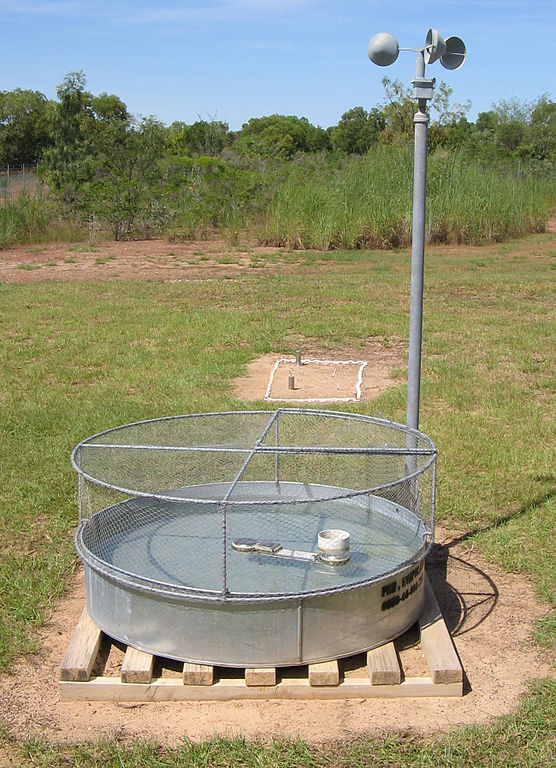
\includegraphics[height=8cm]{evappan}
\emph{(image: \href{https://commons.wikimedia.org/wiki/File:Evaporation_Pan.jpg}{Bidgee, Wikipedia)}}

An evaporation pan is placed in a location with an ambient air temperature of \SI{300}{\kelvin} and relative humidity of 25\%. The pan contains water at the same temperature as the surrounding air. The pan has a diameter of \SI{20}{\cm} and height of \SI{160}{\mm}, and it starts half-full of water.

1. Assuming only diffusive mass transport, what is the initial evaporation rate?

2. Including the effects of advection, what is the initial evaporation rate?

%3. Determine how long it takes for all the water to evaporate.

\subsection*{Solution}
1. \SI{1.087e-8}{\kilo\mol\per\second}\\
2. \SI{1.108e-8}{\kilo\mol\per\second}





\newpage
\section{Stationary Medium}

\subsection*{Resources}
\begin{itemize}
    \item Video: \url{https://www.youtube.com/watch?v=F0deXOH_YEM}
\end{itemize}

\subsection*{Challenge}
\begin{enumerate}
    \item Briefly explain what is meant by a stationary medium.
    \item Considering a stationary medium of 3 species ``A'', ``B'' and ``C'', if the flux of species ``A'' is \SI{2}{\kmol\per\square\meter\per\second} and ``B'' is \SI{-8}{\kmol\per\square\meter\per\second}, what is the flux of species ``C''?
    \item Considering a binary system of atoms ``A'' and ``B'' with concentration \SI{5}{\kmol\per\cubic\meter} and \SI{10}{\kmol\per\cubic\meter} respectively, if the molar velocity of species ``A'' is \SI{2}{\meter\per\second}, what is the molar velocity of species ``B''?
\end{enumerate}



\subsection*{Solutions}
1. Please compare your answer with your partner

2. (enter to two decimal places in units of \si{\kmol\per\square\meter\per\second}) \hash{g}{2c32d8}

3. (enter to two decimal places in units of \si{\meter\per\second}) \hash{h}{3ccbb4}




\newpage
\section{Stationary Medium Approximation}

\subsection*{Resources}
\begin{itemize}
    \item Book 14.3
\end{itemize}

\subsection*{Challenge}
In a few sentences, describe what is meant by \emph{the stationary medium approximation}. Give at least one real-world example each of case where the stationary medium approximation would and would-not be appropriate.

\subsection*{Solution}
Compare your answer with your partner




\newpage
\section{Steady-state definition}

\subsection*{Resources}
\begin{itemize}
    \item Web: \url{http://www.virginia.edu/bohr/mse209/chapter5.htm}
\end{itemize}

\subsection*{Challenge}
The example in section 14.4.3 talks of steady state conditions.

1. Write a sentence or two explaining what is meant by steady-state conditions in this context.

2. What is $\delta J(x) / \delta t$ at any given position $x$ under a steady-state condition?

\subsection*{Solutions}
1. Please compare your answer with your partner

2.\\
X = Your solution\\
Form: Decimal, to 1 decimal place\\
Place the indicated letter in front of the number\\
Example: aX where $X=42.5$ is entered as \href{http://www.wolframalpha.com/input/?i=md5+hash+of+\%22a42.5\%22}{a42.5}

hash of aX = 9497cd




\newpage
\section{Steady-state diffusion planer example I}

\subsection*{Resources}
\begin{itemize}
    \item Book: 14.4.1 to 14.4.3
    \item Video: \url{https://youtu.be/4KACai1gYzc}
\end{itemize}

\subsection*{Challenge}
Work through the calculation from equations 14.51 to 14.54, showing your reasoning along the way. Don't worry about the concept of diffusion resistance for now.




\newpage
\section{Steady-state diffusion planer example II}

\subsection*{Resources}
\begin{itemize}
    \item Book: 14.4.1 to 14.4.3
    \item Video: \url{https://youtu.be/4KACai1gYzc}
\end{itemize}

\subsection*{Challenge}
Work through example 14.3 in section 14.4.3.




\newpage
\section{Steady-state diffusion through flat surface}

\subsection*{Resources}
\begin{itemize}
    \item Book: 14.4.1 to 14.4.3
\end{itemize}

\subsection*{Challenge}
A thin plastic membrane is used to maintain separation between helium and an outer chamber. Under steady-state conditions, the concentration of helium is \SI{0.02}{\kmol\per\cubic\meter} and \SI{0.005}{\kmol\per\cubic\meter} at the inner and outer boundaries respectively. If the membrane is \SI{1}{\mm} thick and the binary diffusion coefficient of helium in the plastic membrane is \SI{e-9}{\square\meter\per\second}, what is the diffusive flux through the membrane in terms of \si{\kmol\per\second\per\square\meter} and \si{\kg\per\second\per\square\meter}?

\subsection*{Solution}
\SI{1.5e-8}{\kmol\per\second\per\square\meter}\\
\SI{6.0e-8}{\kg\per\second\per\square\meter}




\newpage
\section{Steady-state diffusion in pipe walls}

\subsection*{Resources}
\begin{itemize}
    \item Book: 14.4.1 to 14.4.3
\end{itemize}

\subsection*{Challenge}
A pipe with inner-radius \SI{10}{\cm} and outer-radius \SI{13}{\cm} is carrying hydrogen. The concentration of hydrogen inside the pipe is \SI{0.07}{\kmol\per\cubic\meter} and outside the pipe is \SI{0.04}{\kmol\per\cubic\meter}. If the hydrogen has a diffusion coefficient of \SI{e-8}{\square\meter\per\second} in the walls of the pipe, at what rate is hydrogen lost from the pipe, per metre length of pipe?

\subsection*{Solution}
\SI{7.18e-9}{\kmol\per\second}




\newpage
\section{Raoult's law}

\subsection*{Resources}
\begin{itemize}
    \item Book: 14.5.1
\end{itemize}

\subsection*{Challenge}
Considering a puddle of water exposed to the atmosphere at \SI{17}{\celsius}, calculate:

1. The molar fraction of water vapour on the air-side of the water-air interface.\\
2. The mass fraction of water vapour on the air-side of the water-air interface.\\
3. The molar fraction of water vapour on the water-side of the water-air interface.\\
4. The mass fraction of water vapour on the water-side of the water-air interface.

\subsection*{Solution}
1. \num{0.019}

2. \num{0.012}

3.\\
X = Your solution\\
Form: Decimal, to 3 decimal places\\
Place the indicated letter in front of the number\\
Example: aX where $X=42.544$ is entered as \href{http://www.wolframalpha.com/input/?i=md5+hash+of+\%22a42.544\%22}{a42.544}

hash of bX = 4b5ab9

4.\\
X = Your solution\\
Form: Decimal, to 3 decimal places\\
Place the indicated letter in front of the number\\
Example: aX where $X=42.544$ is entered as \href{http://www.wolframalpha.com/input/?i=md5+hash+of+\%22a42.544\%22}{a42.544}

hash of cX = 737b49




\newpage
\section{Boundary conditions}

\subsection*{Resources}
\begin{itemize}
    \item Book: First page of section 14.5
\end{itemize}

\subsection*{Challenge}
State two different types of boundary conditions in terms of molar density, $x_i$.

\subsection*{Solution}
Please discuss with your partner and the teacher.




\newpage
\section{Henry's law}

\subsection*{Resources}
\begin{itemize}
    \item Book: 14.5.2
\end{itemize}

\subsection*{Challenge}
Consider a gas stream flowing above a liquid. Species $A$ has a mole fraction of \num{0.5} in the liquid while species $B$ has a mole fraction of \num{0.005} in the liquid.Calculate Henry's constant for the gas where Henry's law is most applicable, if the partial pressure of both species in the gas stream is \SI{0.5}{\bar}.

\subsection*{Solution}
\hashnew{1}{}{5}{f}{4e930b} % Decimal places, ``s'' in places, 42.X, hash letter, hash




\newpage
\section{Solubility}

\subsection*{Resources}
\begin{itemize}
    \item Book: 14.5.2
\end{itemize}

\subsection*{Challenge}
1. Considering a solid-gas interface, calculate the solubility of species \emph{A} if the density of \emph{A} is \SI{e-3}{\kmol\per\cubic\meter} in the solid given a partial pressure of \SI{0.5}{\bar} in the gas.

2. What volume will species \emph{A} occupy in the gas-phase at STP if it occupies \SI{20}{\cubic\meter} in the solid phase?

\subsection*{Solution}
1.\\
X = Your solution\\
Units: kmol / $m^3$ (solid) / bar (partial pressure in gas phase)\\
Form: Scientific notation with the mantissa in standard form to 1 decimal place and the exponent in integer form\\
Place the indicated letter in front of the number\\
Example: aX where $X=4.0 \times 10^{-3}$ is entered as \href{http://www.wolframalpha.com/input/?i=md5+hash+of+\%22a4.0e-3\%22}{a4.0e-3}

hash of gX = 0174a0

2. \SI{0.908}{\cubic\meter}




\newpage
\section{Flux through membrane with solubility}

\subsection*{Resources}
\begin{itemize}
    \item Book: 14.5.2
\end{itemize}

\subsection*{Challenge}
Work through example 14.4




\newpage
\section{Flux through spherical membrane}

\subsection*{Resources}
\begin{itemize}
    \item Book: 14.5.2
\end{itemize}

\subsection*{Challenge}
Consider helium gas stored in a silicon spherical container at \SI{25}{\celsius} and \SI{4}{\bar} pressure, with an inner radius of \SI{100}{\mm} and outer radius of \SI{110}{\mm}. Assume a diffusion coefficient of helium in the walls of the container of \SI{0.4e-13}{\square\meter\per\second} and a solubility of Helium in Silicon of \SI{4.5e-4}{\kmol\per\cubic\meter\per\bar}. Since the thickness of the walls is similar to the radius, you cannot approximate the surface as being flat, as was done in the previous challenge. In particular, the surface area is now a function of radius.

\subsection*{Solution}
\SI{4e-15}{\kg\per\second}


\appendix 
\chapter{Supporting challenges}
\newpage
\section{Partial pressure and humidity}

\subsection*{Challenge}
If the saturation pressure of water in air at a given temperature is \SI{0.02}{\bar} and the relative humidity of the air is 30\%, calculate the partial pressure of the water vapour in the air.

\subsection*{Solution}
X = Your solution\\
Form: Decimal, to 3 decimal places\\
Place the indicated letter in front of the number\\
Example: aX where $X=42.544$ is entered as \href{http://www.wolframalpha.com/input/?i=md5+hash+of+\%22a42.544\%22}{a42.544}

hash of dX = f8dcaa



\newpage
\section{Pressure and molar density}

\subsection*{Challenge}
Given that the saturation pressure of water in air at a given temperature is \SI{0.05}{\bar} with a saturated molar density of \SI{5}{\kmol\per\cubic\meter}, if the partial pressure of water in the air is \SI{0.01}{\bar}, calculate the molar density of the water in the air.

\subsection*{Solution}
X = Your solution\\
Form: Decimal, to 1 decimal place\\
Place the indicated letter in front of the number\\
Example: aX where $X=42.5$ is entered as \href{http://www.wolframalpha.com/input/?i=md5+hash+of+\%22a42.544\%22}{a42.5}

hash of eX = 1c8d37



\newpage
\section{Specific volume}

\subsection*{Challenge}
Referring to the specific volume of saturated water at 290 K in table A-6 ($v_g$), what is the saturated molar concentration? You cannot assume this is an ideal gas.

\subsection*{Solution}
\SI{7.97e-4}{\kmol\per\cubic\meter}




\newpage
\section{Molar density of air}

\subsection*{Challenge}
Assuming air to be an ideal gas, calculate the molar density of air, $C_{air}$ at 300 K and atmospheric pressure.

\subsection*{Solution}
\SI{4.1e-2}{\kmol\per\cubic\meter}


\end{document}
